 
%%%%%%%%%%%%%%%%%%%%%%%%%%%%%%%%%%%%%%%%%%%%%%%%%%%%%%%%%%%%%%%%%%%%%%%%
%%%%%% COMMON NEIGHBORS
%%%%%%%%%%%%%%%%%%%%%%%%%%%%%%%%%%%%%%%%%%%%%%%%%%%%%%%%%%%%%%%%%%%%%%%%

\section{Bestimmung der gemeinsamen Nachbarschaft}

\textcolor{red}{Wie bereits erwähnt} müssen um einen \textcolor{red}{Curveball-Tausch} auf den Knoten $u$ und $v$
auszuführen die Nachbarschaften der beiden Knoten bekannt sein. Dabei sind die Knoten gesucht, 
welche jeweils nur entweder $u$ oder $v$ als Nachbarn haben, also in der \textcolor{red}{disjunkten Nachbarschaft (kann man das sagen?)} liegen.
Um diese Knoten zu finden, kann man jedoch einfach die gemeinsame Nachbarschaft bestimmen. Die Knoten
in der disjunkten Nachbarschaft sind dann alle Nachbarn von $u$ und $v$, welche\textcolor{red}{VORSORTIERT}
 nicht in der gemeinsamen
Nachbarschaft liegen. 
\\
Als Datenstruktur liegen uns die Nachbarschaften in einer Art \textcolor{red}{Adjazenzliste (naja eine Liste ist es ja nicht wirklich)}
vor, sodass es für jeden Knoten des Graphen einen Vektor gibt, indem die Nachbarn gespeichert sind.
Um nun gemeinsame Nachbarn
zweier Knoten zu bestimmen, muss man also nur herausfinden, welche Einträge in beiden Vektoren gemeinsam
vorkommen. Dafür gibt es verschiedene Varianten, die 
im Folgenden erklärt werden.
\\
\\
Als ersten ''naiven'' Ansatz könnte man für jedes Element des Vektors $u$ den gesamten anderen 
Vektors $v$ per linearer Suche nach diesem Element durchsuchen. Hierfür ergibt sich eine Laufzeit von
$\O(|u|\cdot|v|)$, was aber natürlich nicht sehr sinnvoll ist, da der Vektor $v$ ziemlich oft 
durchlaufen werden muss und wir 
im Falle von massiven Graphen davon ausgehen können, dass die Vektoren (also die Nachbarschaften)
ziemlich groß werden. 
\\
Um dieses Problem zu verhindern kann man beide Vektoren aufsteigend sortieren. Um nun zu herauszufinden,
welche Werte in beiden Vektoren vorkommen, muss man lediglich $u$ und $v$ gleichzeitig linear durchlaufen
und testen, ob die Werte gleich sind. Somit muss man jedes Element der beiden Vektoren - nach dem Sortieren - 
nur einmal betrachten, was offensichtlich zu einer verbesserten Laufzeit im Vergleich zum ''naiven''
Ansatz führt. Man erhält damit eine Laufzeit von $\O(|u|\cdot \log (|u|)  + |v|\cdot\log(|v|))$. 
Diese Variante wird im Folgenden als \SorSor \textcolor{red}{(darf ich das in
englisch lassen?)} bezeichnet.
\\
Dies kann man leicht abwandeln zur Variante \SorSea. Dabei wird nur der größere Vektor (z.B. $u$)
sortiert.
Für jedes Element des kleineren Vektors wird nun per binärer Suche geprüft, ob das Element auch im 
größeren Vorhanden ist. Analog zu dieser Variante gibt es noch \SeaSor, bei welcher 
der kleinere Vektor sortiert wird. \textcolor{red}{LZ?}
\\
Eine weitere Methode um  viele Werte schnell zu durchsuchen, bietet die Datenstruktur \textit{Set}.
Dabei wird jedes Element des einen Vektors (z.B. $u$) in das Set eingefügt. Die Datenstruktur
baut aus diesen Elementen dann einen Binären Suchbaum. Für jedes Element aus $v$ kann nun in logarithmischer
Zeit bestimmt werden, ob es im Set und somit auch in $u$ vorhanden ist. Auch hier gibt es zwei
analoge Varianten, nämlich \SetSea, bei der der größere Vektor in das Set eingefügt wird
und \SeaSet, bei der der kleinere Vektor zum Set hinzugefügt wird.
\\
Die letzte Methode, die \textcolor{red}{wir (darf ich ''wir'' sagen?!)} an dieser Stelle betrachten,
ist die Verwendung der Datenstruktur \textit{unordered\_set}. Diese ist sehr ähnlich wie Set, mit
dem Unterschied, dass die Werte nicht in geordneter Reihenfolge gespeichert werden, sondern
in einer \textcolor{red}{Hash-Tabelle?}. Ebenfalls gibt es hierbei wieder die Varianten, 
in denen der größere Vektor in das unordered\_set eingefügt wird (\USetSea) 
oder der kleinere (\SeaUSet).
\\
\\
Wir haben also insgesamt sieben verschiedene Möglichkeiten, die alle eine ähnliche Laufzeit \textcolor{red}{(wirklich?!)}
haben. Somit muss experimentell herausgefunden werden, welche dieser Varianten für welche Instanzen am
schnellsten sind. Weiterhin testen wir noch, ob die Invariante, dass die Vektoren bereits 
sortiert sind, zu einer besseren Laufzeit führt.


\textcolor{red}{Pseudocode zu den einzelnen Varianten?}\\
\textcolor{red}{LAUFZEIT ??}



%%%%%%%%%%%%%%%%%%%%%%%%%%%%%%%%%%%%%%%%%%%%%%%%%%%%%%%%%%%%%%%%%%%%%%%%
%%%%%% Nachbarn Tauschen
%%%%%%%%%%%%%%%%%%%%%%%%%%%%%%%%%%%%%%%%%%%%%%%%%%%%%%%%%%%%%%%%%%%%%%%%

\section{Tauschen der Nachbarn}
Im vorherigen Teil wurde beschrieben, wie man die gemeinsame und die disjunkte Nachbarschaft zweier Knoten
$u$ und $v$ bestimmt. Nun beschäftigen wir uns damit, wie man diese Knoten zufällig tauscht. Als Eingabe 
stehen die Vektoren $d$, welcher alle Knoten aus der disjunkten Nachbarschaft enthält
und $c$, der die gemeinsamen Nachbarn enthält, zur Verfügung. Weiterhin seien $\text{deg}(u)$ und
 $\text{deg}(v)$ die ursprünglichen Knotengrade. 
Wir betrachten hierfür zwei Möglichkeiten.
\\
\\
Die erste Idee besteht darin,  
den Vektor der disjunkten Nachbarn zufällig zu permutieren, sodass jedes Element an 
einer zufälligen Position steht. Um nun die beide ''neuen'' Nachbarschaften von $u$ und $v$ zu erstellen,
werden zuerst die Knoten aus der gemeinsamen Nachbarschaft in die \textcolor{red}{(leeren)} Vektoren von $u$ und $v$ kopiert.
Dann werden die ersten Elemente aus dem permutierten Vektor in den kleineren aus $u$ und $v$ kopiert.
Dabei werden genau so viele Elemente kopiert, dass dieser wieder die gleiche Größe hat wie vor dem Beginn
des Tausches. Die restlichen Elemente aus dem disjunkten Vektor werden schließlich in den anderen Vektor kopiert.
Zur besseren Veranschaulichung ist in Abbildung \ref{fig:trade_shuffle} ein Beispiel zu sehen.
\begin{figure}[h]
\centering
  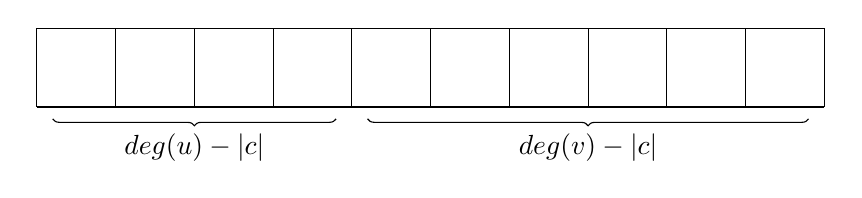
\begin{tikzpicture}[decoration=brace]
    % Die Grundlinie:
    \draw(0,0)--(10,0);
    \draw(0,1)--(10,1);

    % Striche und Beschriftung in Abständen 0, 2, 4, 6, ...
    \foreach \x/\xtext in {0,1,2,3,4,5,6,7,8,9,10}
      \draw(\x,0)--(\x,1) node[below] {};
      
    % untere geschweifte Klammer mit Text darunter:
    \draw[decorate, yshift=-1ex] (3.8,0) -- node[below=0.4ex] {$\text{deg}(u) - |c|$} (0.2,0);

    \draw[decorate, yshift=-1ex] (9.8,0) -- node[below=0.4ex] {$\text{deg}(v) - |c|$} (4.2,0);

  \end{tikzpicture}
  \caption{\textcolor{red}{ist das Beispiel unnötig?}}
  \label{fig:trade_shuffle}
\end{figure}
Die Kästchen stellen die Elemente des permutierten Vektors $d$ dar. Ohne Beschränkung der
Allgemeinheit betrachten wir den Fall, dass die Nachbarschaft von $u$ die kleinere ist, also dass 
$\text{deg}(u) \le \text{deg}(v)$ gilt. Somit werden die ersten $\text{deg}(u)-|c|$ Elemente zum 
Vektor $u$ hinzugefügt. Die restlichen
Elemente werden folglich in $v$ kopiert.
Die Größen von $u$ und $v$ - also dementsprechend die Knotengrade der beiden Knoten - haben sich durch das
zufällige Tauschen der disjunkten Nachbarn offensichtlich
nicht verändert.
\\
Bei die diesem Verfahren fällt  jedoch auf, dass einige Elemente beim Permutieren unnötig vertauscht werden.
Für jedes Element ist es eigentlich nur entscheidend, ob es unter den ersten $\text{deg}(u)$  liegt (also zum Vektor
$u$ hinzugefügt wird) oder nicht. Auf welcher Position genau es in diesen Bereichen liegt, ist egal. Man
kann also die Laufzeit dieser Variante verbessern, indem nicht der ganze Vektor zufällig permutiert 
wird, sondern nur die ersten $\text{deg}(u)$ Elemente zufällig gewählt werden. Dies macht die Funktion 
\textcolor{red}{\textit{random\_bipartition\_shuffle}}.
\\
Ein Nachteil bei dieser Methode ist, dass durch das zufällige Vertauschen die beiden Vektoren
$u$ und $v$ nicht mehr sortiert sind. Damit wird die im vorherigen \textcolor{red}{kapitel?} beschriebene
Invariante eventuell verletzt. Um die Invariante aufrecht zu halten muss man also als letzten Schritt
die beiden Vektoren nochmals sortieren.
Wir nennen diese Variante \perm
\\
\\
Die zweite Möglichkeit die wir betrachten heißt \distr.
\\
Die Idee besteht dabei, dass wir über jedes Element des Vektors $d$ iterieren und eine Wahrscheinlichkeit
berechnen, mit
der das Element in den Vektor $u$ (beziehungsweise $v$) eingefügt werden soll. Dann wird in einem 
Bernoulli Experiment mit genau dieser Wahrscheinlichkeit ein Zufallsbit gezogen. Je nachdem, welchen
Wert das Zufallsbit hat, wird das Element dann entweder in $u$ oder in $v$ kopiert. Dies wird so lange
wiederholt, bis einer der beiden Vektoren seine maximale Kapazität erreicht hat. 
\\
Um die Wahrscheinlichkeit zu berechnen werden am Anfang zwei Variablen $n_v$ und $n_u$ initialisiert, 
welche den Kapazitäten der beiden Vektoren $u$ und $v$ entsprechen, wenn die Elemente aus der 
gemeinsamen Nachbarschaft nicht berücksichtigt werden. Es gilt also $n_v = \text{deg}(v) - |c|$ und
$n_u= \text{deg}(u) - |c|$.
Damit hat das erste Element des Vektors $d$ eine Wahrscheinlichkeit von $p_u = \frac{n_u}{n_u+n_v}$, dem
Vektor $u$ hinzugefügt zu werden und analog eine Wahrscheinlichkeit $p_v = \frac{n_v}{n_u+n_v}$, um
in $v$ zu gelangen. Offensichtlich gilt $p_u + p_v = 1$. Dann wird mit einer der beiden
Wahrscheinlichkeiten das Bernoulli Experiment durchgeführt, wobei es egal ist, welche Wahrscheinlichkeit
man dazu wählt, da $p_u$ genau die Gegenwahrscheinlichkeit von $p_v$ ist und umgekehrt. 
Wählt man beispielsweise $p_u$ und das Experiment liefert eine eins, dann wird das aktuelle Element
in den Vektor $u$ kopiert. Dabei
hat sich aber offensichtlich die verbleibende Kapazität des Vektors $u$ verringert. Also muss
der Wert $n_u$ dekrementiert werden. Analoges gilt, falls das Element in den Vektor $v$ kopiert wird.
Somit ändern sich nach jeder Iteration die Wahrscheinlichkeiten $p_u$ beziehungsweise $p_v$.
Gilt nach irgendeinem Zeitpunkt entweder $n_u = 0$ oder $n_v = 0$, ist offenbar einer der Vektoren 
keine Kapazität mehr frei. Somit werden die übrigen Elemente, die noch in $d$ vorhanden sind, 
einfach dem anderen Vektor hinzugefügt.
\\
Ein Vorteil dieser Methode ist, dass die beschriebene Invariante aufrecht erhalten werden kann.
War der Vektor der disjunkten Nachbarschaft vor Beginn dieser Methode aufsteigend sortiert,
dann sind auch die bisherigen Elemente der Vektoren $u$ und $v$ aufsteigend sortiert, da für jedes
Element nacheinander entschieden wurde, ob es zu $u$ oder zu $v$ hinzugefügt wird und dabei die
Reihenfolge der Elemente untereinander nicht verändert wurde.
\\
Zum Schluss müssen noch die die gemeinsamen Nachbarn zu den Vektoren $u$ und $v$ hinzugefügt werden.
Möchte man die Invariante aufrecht erhalten, dann sind die beiden Vektoren wie beschrieben schon
aufsteigend sortiert. Da auch die Elemente aus $c$ aufsteigend sortiert sind, erhält man
die endgültigen Vektoren von $u$ und $v$ durch ein Mergen mit $c$. Soll die Invariante jedoch
nicht aufrecht erhalten werden, reicht es aus, die Elemente aus $c$ an das Ende der beiden Vektoren
zu kopieren.


%%%%%%%%%%%%%%%%%%%%%%%%%%%%%%%%%%%%%%%%%%%%%%%%%%%%%%%%%%%%%%%%%%%%%%%%
%%%%%% Global Curveball Tausch
%%%%%%%%%%%%%%%%%%%%%%%%%%%%%%%%%%%%%%%%%%%%%%%%%%%%%%%%%%%%%%%%%%%%%%%%


\section{Globaler Curveball Tausch}
Wie in den beiden vorherigen \textcolor{red}{Abschnitten} beschrieben, besteht ein Curveball Tausch auf zwei Knoten $u$ und $v$ daraus, die gemeinsame und disjunkte Nachbarschaft der beiden Vektoren zu bestimmen
und schließlich die Knoten aus der disjunkten Nachbarschaft zufällig zu tauschen.
\\
Bei einem Globalen Curveball Tausch, werden mehrere Curveball-Tausche gleichzeitig ausgeführt.
Hierbei wird ausgenutzt, dass wir ausschließlich bipartite Graphen betrachten \textcolor{red}{echt?}


\red{INVRIANTE NAME?!}


\textcolor{red}{wie wir in kapitel xxx sehen, sind die varianten blblal am schnellsten. daher gehen wir 
an dieser stelle nochmals auf diese methoden ein indem wir sie im Pseudocode beschreiben}


\begin{table}
	\centering
	\begin{tabular}{c||c|c||c|c}
		 & \multicolumn{2}{c||}{\distr} & \multicolumn{2}{c}{\perm} \\
		 & \true & \false & \true & \false
		\\ \hline\hline
		\SorSor & & & & \\ \hline\hline
		\SeaSor & & & &\\ \hline\hline
		\SorSea & & & &\\ \hline\hline
		\SeaSet & & & &\\ \hline\hline
		\SetSea & & & &\\ \hline\hline
		\SeaUSet & & & &\\ \hline\hline
		\USetSea& & & &
	\end{tabular}
	\label{tab:varianten_curveball_tausch}
	\caption{Jedes Feld in der Tabelle entspricht einer Variante für einen \ct}
\end{table}

%\section{\red{Pseudocode}}

\begin{algorithm}
  \caption{SortSort}\label{algo:sortsort}
  \begin{algorithmic}[1]
    \Procedure{SortSort}{$u,v$}%\Comment{The g.c.d. of a and b}
	  \State U $ \gets N(u)$ \Comment{Nachbarschaft von u}
	  \State V $ \gets N(v)$ \Comment{Nachbarschaft von v}
	  %\State
	  \State \texttt{sort(}U\texttt{)} \label{algo:inv1} \Comment{Sortiere beide Vektoren}
	  \State \texttt{sort(}V\texttt{)} \label{algo:inv2}
	  %\State
	  \State nu $\gets 0$ \Comment{Zähler für U}
	  \State nv $\gets 0$ \Comment{Zähler für V}
	  
      \While{(nu < U.\texttt{size()}) and (nv < V.\texttt{size()})}
        \If{U[nu] < V[nv]}
			\State disjoint.\texttt{append(}U[nu]\texttt{)}
			\State nu ++
			\ElsIf{U[nu] > V[nv]}
				\State disjoint.\texttt{append(}V[nv]\texttt{)}
				\State nv ++
			\ElsIf{U[nu] == V[nv]}
				\State common.\texttt{append(}U[nu]\texttt{)}
				\State nu ++
				\State nv ++
        \EndIf
      \EndWhile\label{euclidendwhile}
      \If{nu $\neq$ U.\texttt{size()}}
			\State disjoint.\texttt{append(} U[nu], U[nu+1], \dots\texttt{)}
			\Else{}
			\State disjoint.\texttt{append(} V[nv], V[nv+1], \dots\texttt{)}
      \EndIf
      \State \textbf{return} common, disjoint
   \EndProcedure
  \end{algorithmic}
\end{algorithm}


%\red{bei vorsortiert fällt Zeile \ref{algo:inv1} und \ref{algo:inv2} raus!!}
%\\
%\\
%\red{Distribution}

\begin{algorithm}[h]
\begin{algorithmic}[1]
\Procedure{Distribution}{common, disjoint}
	\State nu $\gets$ U.\texttt{size()} - common.\texttt{size()}
	\State nv $\gets$ V.\texttt{size()} - common.\texttt{size()}
	\State i = 0
	\While{i < disjoint.\texttt{size()}}
		\State X $\sim \mathcal{B}(\frac{\text{nu}}{\text{nu}+\text{nv}})$  \Comment{ziehe ein Zufallsbit Bernoulli verteilt mit Wahrscheinlichkeit $\frac{nu}{nu+nv}$}

		\If{X==1}
			\State U.\texttt{append(}disjoint[i]\texttt{)}
			\State i++
			\State nu- -
		\Else{} 
			\State V.\texttt{append(}disjoint[i]\texttt{)}
			\State i++
			\State nv- -
		\EndIf{}
	\EndWhile{}	
	\State U.\texttt{insert(}common\texttt{)}
	\State V.\texttt{insert(}common\texttt{)}
	\State \textbf{return} U, V
\EndProcedure
\end{algorithmic}
	\caption{Distribution}
\end{algorithm}

